\chapter{Diagramas dinâmicos}

Este capítulo apresenta os diagramas comportamentais do Sistema de Gestão de Clínica (SGC), evidenciando como os seus componentes interagem ao longo do tempo e como as entidades centrais transitam entre estados durante a execução dos fluxos de negócio. São empregados três tipos de diagramas: \textbf{diagramas de sequência}, que detalham a ordem cronológica da troca de mensagens entre objetos nos fluxos críticos; \textbf{diagramas de estados}, que modelam o ciclo de vida de entidades-chave, explicitando os estados possíveis e os eventos que disparam cada transição; e \textbf{diagramas de atividades}, que representam processos de negócio mais complexos por meio de raias, permitindo visualizar decisões e a distribuição de responsabilidades entre os atores.

% ---------------------------------------------------------
% Diagramas de Sequência
% ---------------------------------------------------------
\section{Diagramas de Sequência}

Os diagramas de sequência a seguir detalham a ordem cronológica das interações entre objetos participantes para os fluxos de maior criticidade e frequência do SGC. A notação \texttt{objeto:Classe} identifica instâncias concretas colaborando para realizar o caso de uso. Grupos de \textit{transação atômica} delimitam as operações que devem ocorrer de forma indivisível para garantir a integridade dos dados.

Nesta seção, primeiro são descritos todos os modelos de sequência apresentados. Em seguida, os respectivos diagramas são exibidos em sequência, um após o outro, para evitar páginas com pouco conteúdo textual e melhorar a organização visual do capítulo.

São apresentados três fluxos: agendamento de consulta (M-V1-01), dispensação de medicamentos (M-V1-02) e faturamento de atendimento (M-V1-03).

% ---------------------------------------------------------
% Descrição Modelo 1
% ---------------------------------------------------------
\subsection{Modelo M-V1-01 -- Sequência de Agendamento}

O modelo M-V1-01 descreve a sequência de interações entre os objetos participantes no fluxo de agendamento de consulta. A notação \texttt{objeto:Classe} identifica instâncias concretas que colaboram para realizar o caso de uso.

\begin{itemize}
    \item \textbf{autorizacaoService:AutorizacaoService}: verifica se o usuário possui papel (\textit{role}) que permite criar agendamentos.
    \item \textbf{agendaService:AgendaService}: isola a lógica de disponibilidade de horários.
    \item \textbf{Grupo transação atômica}: garante que a reserva do horário e o registro de auditoria ocorram de forma indivisível.
\end{itemize}

% ---------------------------------------------------------
% Descrição Modelo 2
% ---------------------------------------------------------
\subsection{Modelo M-V1-02 -- Sequência de Dispensação}

O modelo M-V1-02 evidencia a colaboração entre controller, serviços de autorização, prescrição, estoque, persistência e auditoria para garantir autorização, validação clínica, baixa de estoque, persistência e rastreabilidade.

% ---------------------------------------------------------
% Descrição Modelo 3
% ---------------------------------------------------------
\subsection{Modelo M-V1-03 -- Sequência de Faturamento}

O modelo M-V1-03 descreve a sequência de interações entre os objetos participantes no fluxo de faturamento de atendimento, correspondente ao caso de uso UC08 — Faturar Atendimento. O diagrama evidencia a colaboração entre o controller de faturamento, os serviços de autorização, consulta e convênio, e os repositórios de persistência e auditoria, garantindo autorização, cálculo de cobertura, geração atômica da conta médica com seus itens e rastreabilidade da operação.

\begin{itemize}
    \item \textbf{faturamentoCtrl:FaturamentoController} --- orquestra o fluxo de faturamento, delegando validação, cálculo e persistência aos serviços especializados.
    \item \textbf{autorizacaoSvc:AutorizacaoService} --- verifica se o usuário possui o papel (\textit{role}) que permite faturar atendimentos.
    \item \textbf{consultaRepo:ConsultaRepository} --- recupera os dados da consulta finalizada, incluindo serviços realizados e convênio associado.
    \item \textbf{convenioSvc:ConvenioService} --- calcula os valores de cobertura e a parte particular do paciente com base no convênio vigente.
    \item \textbf{contaMedicaRepo:ContaMedicaRepository} --- persiste a \texttt{ContaMedica} e os \texttt{ItemContaMedica} de forma atômica.
    \item \textbf{Grupo transação atômica} --- garante que a geração da conta e o registro de auditoria ocorram de forma indivisível.
\end{itemize}

Os diagramas correspondentes aos modelos descritos são apresentados a seguir.

% ---------------------------------------------------------
% Descrição Modelo 4
% ---------------------------------------------------------
\subsection{Modelo M-V1-04 -- Sequência de Atendimento Clínico}

O modelo M-V1-04 descreve a sequência de interações entre os objetos participantes no fluxo de realização do atendimento clínico, correspondente ao caso de uso UC04 --- Realizar Atendimento Clínico. O diagrama evidencia a colaboração entre o controller de atendimento, os serviços de autorização, atendimento e auditoria, e os repositórios de consulta, prontuário e atendimento, garantindo autorização, abertura transacional do atendimento, registro da evolução clínica e encerramento rastreável.

\begin{itemize}
    \item \textbf{atendimentoCtrl:AtendimentoController} --- orquestra o fluxo de atendimento, delegando validação, criação e encerramento aos serviços especializados.
    \item \textbf{autorizacaoSvc:AutorizacaoService} --- verifica se o usuário possui o papel (\textit{role}) que permite realizar atendimentos.
    \item \textbf{consultaRepo:ConsultaRepository} --- recupera a consulta em status \textit{Check-in} e atualiza seu status ao longo do fluxo.
    \item \textbf{prontuarioRepo:ProntuarioRepository} --- recupera o prontuário existente do paciente para exibição do histórico clínico.
    \item \textbf{atendimentoSvc:AtendimentoService} --- encapsula as regras de negócio de abertura, registro de evolução e encerramento do atendimento.
    \item \textbf{atendimentoRepo:AtendimentoRepository} --- persiste o \texttt{Atendimento}, a \texttt{EvolucaoClinica} e as atualizações de status de forma atômica.
    \item \textbf{Grupos de transação atômica} --- garantem que (a) a criação do atendimento e a atualização do status da consulta, e (b) o encerramento e o registro de auditoria ocorram de forma indivisível.
\end{itemize}

% ---------------------------------------------------------
% Descrição Modelo 5 — Autenticação RBAC
% ---------------------------------------------------------
\subsection{Modelo M-V1-05 -- Sequência de Autenticação e Autorização RBAC}

O modelo M-V1-05 descreve a sequência de autenticação e autorização baseada em papéis (RBAC), correspondente ao cenário CN-03. Este fluxo é pré-condição para todos os demais casos de uso do SGC, garantindo que apenas usuários com identidade validada e perfil adequado acessem os módulos do sistema.

\begin{itemize}
    \item \textbf{authCtrl:AuthController} --- recebe as credenciais e orquestra o processo de autenticação.
    \item \textbf{authSvc:AuthService} --- valida credenciais, coordena a verificação de MFA e gera o token de sessão.
    \item \textbf{usuarioRepo:UsuarioRepository} --- recupera o registro do usuário para validação de senha e situação da conta.
    \item \textbf{rbacSvc:RBACService} --- carrega os perfis e permissões associados ao usuário autenticado.
    \item \textbf{permissaoRepo:PermissaoRepository} --- fornece a lista de permissões vinculadas ao perfil do usuário.
    \item \textbf{auditoriaSvc:AuditoriaService} --- registra tentativas de login bem-sucedidas e falhas, em conformidade com C5 e C6 (LGPD).
    \item \textbf{MFA condicional} --- o fluxo de verificação por segundo fator é ativado apenas quando o atributo \texttt{mfaHabilitado} do usuário é verdadeiro.
\end{itemize}

% ---------------------------------------------------------
% Diagrama Modelo 1
% ---------------------------------------------------------
\begin{landscape}
\thispagestyle{plain}
\centering

{\small
\renewcommand{\arraystretch}{1.05}
\begin{tabular}{@{}lp{0.72\linewidth}@{}}
\textbf{View}        & V1 --- Visão de Cenários \\
\textbf{Model Kind}  & UML Sequence Diagram \\
\textbf{Concerns}    & C1 (Controle de Acesso), C4 (Integridade Transacional), C5 (Auditoria), C7 (Modularidade) \\
\textbf{Decisões}    & DA01 (Arquitetura em Camadas), DA03 (RBAC), DA06 (Transações Atômicas), DA07 (Auditoria Centralizada) \\
\end{tabular}
}

\vspace{0.3em}

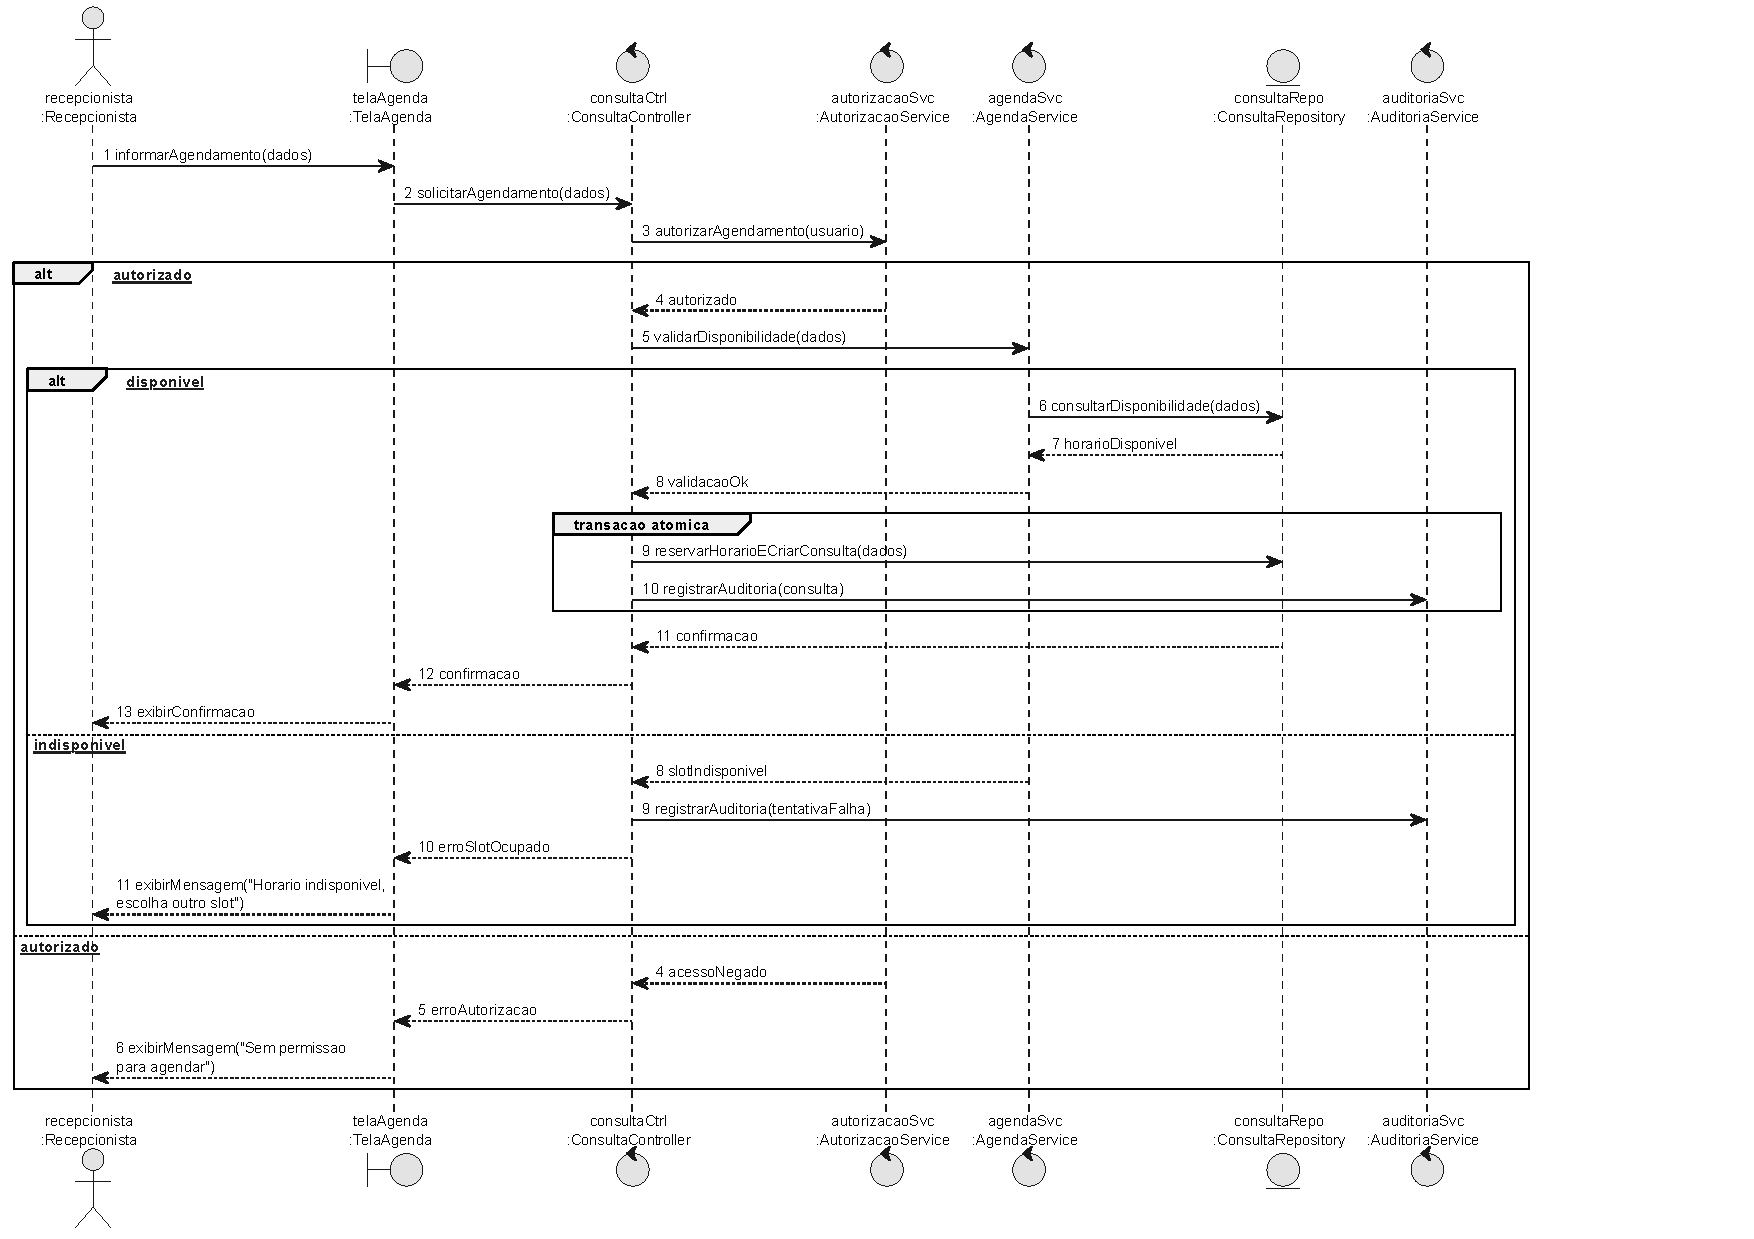
\includegraphics[
    width=0.95\linewidth,
    height=0.66\textheight,
    keepaspectratio
]{Imagens/arquitetura/M-V1-01-sequencia-agendamento}

\captionof{figure}{Modelo M-V1-01 -- Sequência de agendamento de consulta.}
\label{fig:m-v1-01-sequencia-agendamento}

\end{landscape}


% ---------------------------------------------------------
% Diagrama Modelo 2
% ---------------------------------------------------------
\begin{landscape}
\thispagestyle{plain}
\centering

{\scriptsize
\renewcommand{\arraystretch}{1.0}
\begin{tabular}{@{}lp{0.72\linewidth}@{}}
\textbf{View}           & V1 --- Visão de Cenários \\
\textbf{Model Kind}     & UML Sequence Diagram \\
\textbf{Concerns}       & C2 (Desempenho), C4 (Integridade Transacional), C5 (Auditoria), C8 (Interoperabilidade) \\
\textbf{Decisões}       & DA03 (RBAC), DA04 (Persistência Relacional Gerenciada), DA06 (Transações Atômicas), DA07 (Auditoria Centralizada) \\
\textbf{Participantes}  & \texttt{dispensacaoCtrl}: orquestra o fluxo; \texttt{autorizacaoSvc}: verifica permissão; \texttt{prescricaoSvc}: valida a prescrição; \texttt{estoqueService}: valida saldo e baixa estoque; \texttt{dispensacaoRepo}: persiste a dispensação; \texttt{auditoriaSvc}: registra o evento. \\
\end{tabular}
}

\vspace{0.3em}

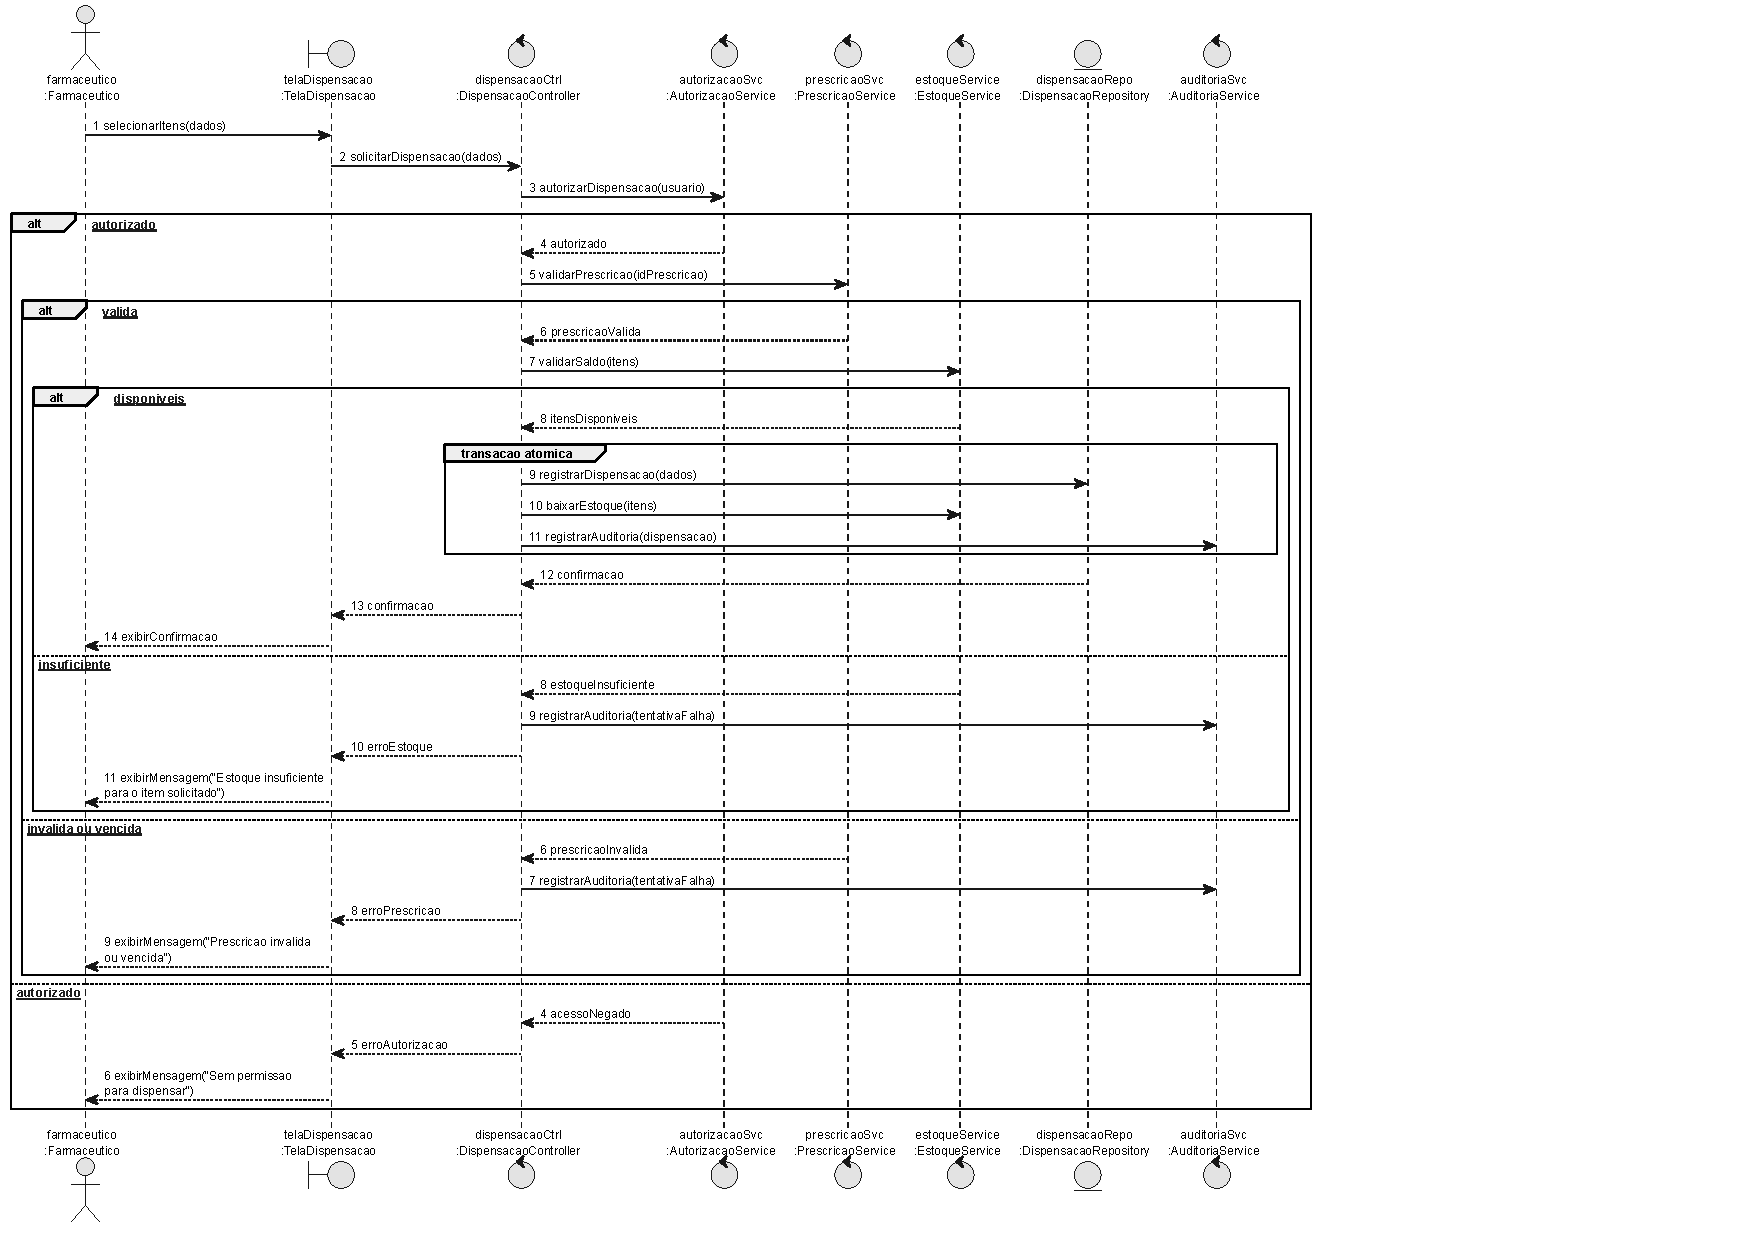
\includegraphics[
    width=0.95\linewidth,
    height=0.60\textheight,
    keepaspectratio
]{Imagens/arquitetura/M-V3-01-sequencia-dispensacao}

\captionof{figure}{Modelo M-V1-02 -- Sequência de dispensação transacional.}
\label{fig:m-v1-02-sequencia-dispensacao}

\end{landscape}


% ---------------------------------------------------------
% Diagrama Modelo 3
% ---------------------------------------------------------
\begin{landscape}
\thispagestyle{plain}
\centering

{\scriptsize
\renewcommand{\arraystretch}{1.0}
\begin{tabular}{@{}lp{0.72\linewidth}@{}}
\textbf{View}           & V1 --- Visão de Cenários \\
\textbf{Model Kind}     & UML Sequence Diagram \\
\textbf{Concerns}       & C1 (Controle de Acesso), C4 (Integridade Transacional), C5 (Auditoria), C9 (Usabilidade) \\
\textbf{Decisões}       & DA03 (RBAC), DA06 (Transações Atômicas), DA07 (Auditoria Centralizada) \\
\textbf{Participantes}  & \texttt{faturamentoCtrl}: orquestra o fluxo; \texttt{autorizacaoSvc}: verifica permissão; \texttt{consultaRepo}: recupera dados da consulta finalizada; \texttt{convenioSvc}: calcula cobertura; \texttt{contaMedicaRepo}: persiste conta e itens; \texttt{auditoriaSvc}: registra o evento. \\
\end{tabular}
}

\vspace{0.3em}

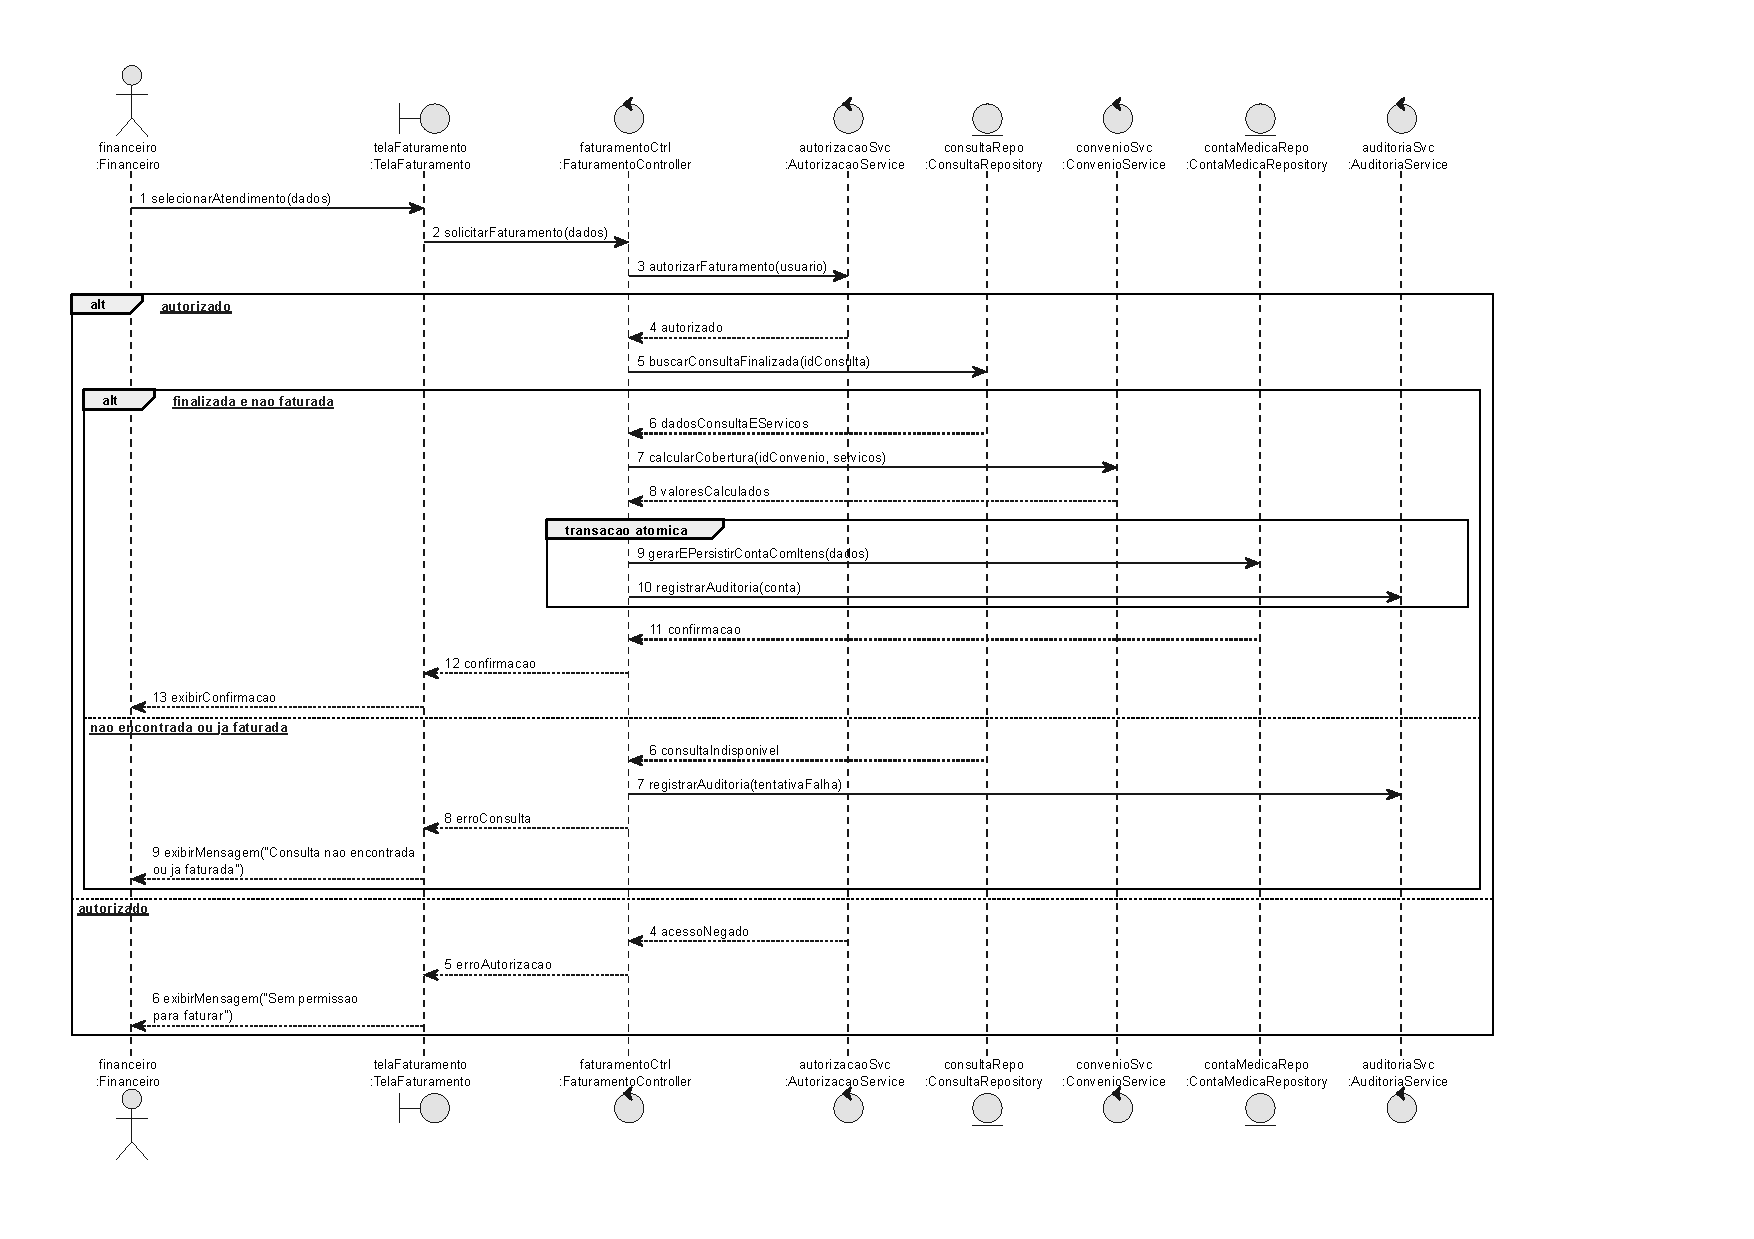
\includegraphics[
    width=0.92\linewidth,
    height=0.58\textheight,
    keepaspectratio,
    trim=0 80 0 0,
    clip
]{Imagens/arquitetura/M-V1-03-sequencia-faturamento}

\captionof{figure}{Modelo M-V1-03 -- Sequência de faturamento de atendimento.}
\label{fig:m-v1-03-sequencia-faturamento}

\end{landscape}


% ---------------------------------------------------------
% Diagrama Modelo 4 — Atendimento Clínico
% ---------------------------------------------------------
\begin{landscape}
\thispagestyle{plain}
\centering

{\scriptsize
\renewcommand{\arraystretch}{1.0}
\begin{tabular}{@{}lp{0.72\linewidth}@{}}
\textbf{View}           & V1 --- Visão de Cenários \\
\textbf{Model Kind}     & UML Sequence Diagram \\
\textbf{Concerns}       & C1 (Controle de Acesso), C4 (Integridade Transacional), C5 (Auditoria), C9 (Usabilidade) \\
\textbf{Decisões}       & DA01 (Arquitetura em Camadas), DA03 (RBAC), DA06 (Transações Atômicas), DA07 (Auditoria Centralizada) \\
\textbf{Participantes}  & \texttt{atendimentoCtrl}: orquestra o fluxo; \texttt{autorizacaoSvc}: verifica permissão; \texttt{consultaRepo}: recupera e atualiza status; \texttt{prontuarioRepo}: fornece histórico clínico; \texttt{atendimentoSvc}: aplica regras de negócio; \texttt{atendimentoRepo}: persiste atendimento; \texttt{auditoriaSvc}: registra eventos. \\
\end{tabular}
}

\vspace{0.3em}

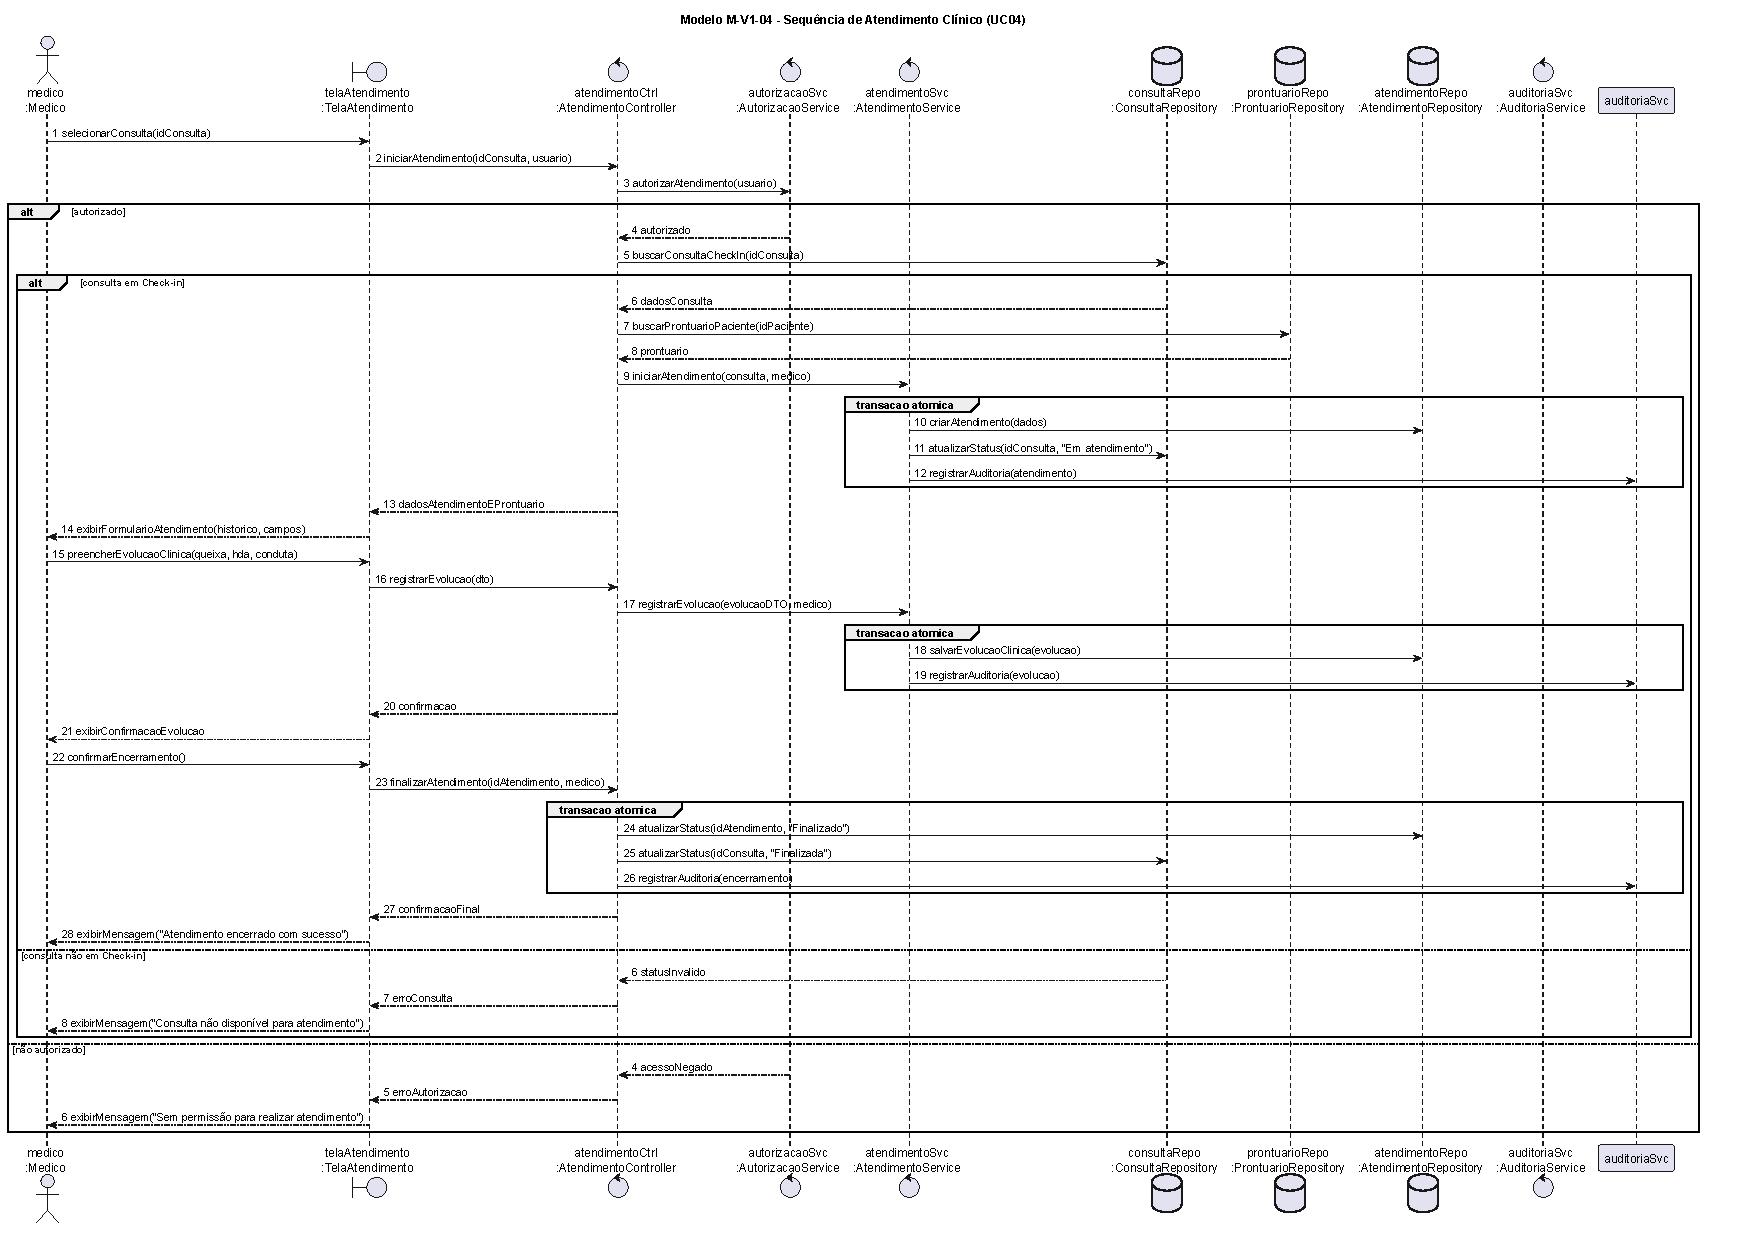
\includegraphics[
    width=0.95\linewidth,
    height=0.58\textheight,
    keepaspectratio
]{Imagens/arquitetura/M-V1-04_Sequencia_Atendimento_Clinico.pdf}

\captionof{figure}{Modelo M-V1-04 -- Sequência de atendimento clínico.}
\label{fig:m-v1-04-sequencia-atendimento}

\end{landscape}


% ---------------------------------------------------------
% Diagrama Modelo 5 — Autenticação RBAC
% ---------------------------------------------------------
\begin{landscape}
\thispagestyle{plain}
\centering

{\scriptsize
\renewcommand{\arraystretch}{1.0}
\begin{tabular}{@{}lp{0.72\linewidth}@{}}
\textbf{View}           & V1 --- Visão de Cenários \\
\textbf{Model Kind}     & UML Sequence Diagram \\
\textbf{Concerns}       & C1 (Controle de Acesso), C5 (Auditoria), C6 (Conformidade com LGPD) \\
\textbf{Decisões}       & DA03 (RBAC), DA07 (Auditoria Centralizada) \\
\textbf{Participantes}  & \texttt{authCtrl}: recebe credenciais e orquestra autenticação; \texttt{authSvc}: valida senha, MFA e gera token; \texttt{usuarioRepo}: recupera dados do usuário; \texttt{rbacSvc}: carrega perfis e permissões; \texttt{permissaoRepo}: fornece permissões; \texttt{auditoriaSvc}: registra tentativas e resultados. \\
\end{tabular}
}

\vspace{0.3em}

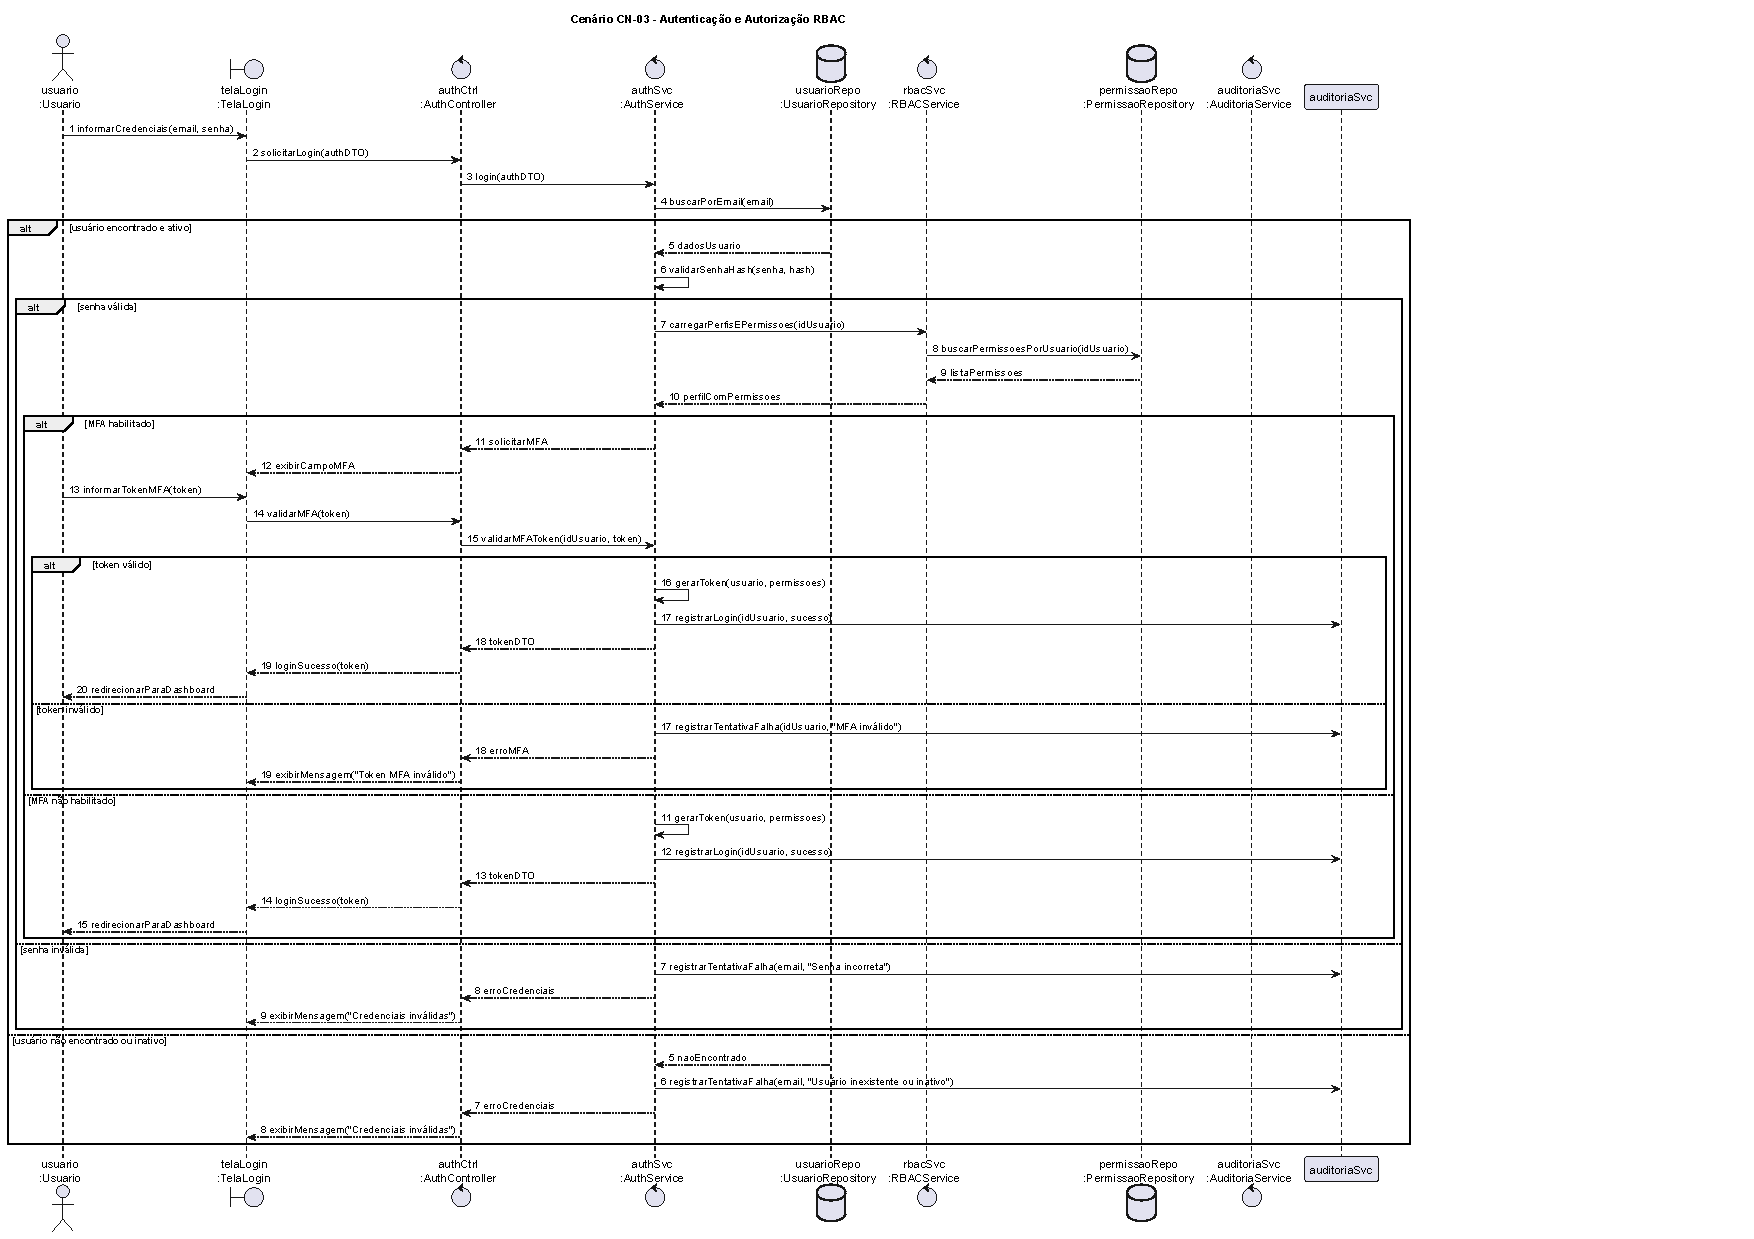
\includegraphics[
    width=0.95\linewidth,
    height=0.58\textheight,
    keepaspectratio
]{Imagens/arquitetura/M-V1-CN03_Sequencia_Autenticacao_RBAC.pdf}

\captionof{figure}{Modelo M-V1-05 -- Sequência de autenticação e autorização RBAC (CN-03).}
\label{fig:m-v1-05-sequencia-autenticacao-rbac}

\end{landscape}

% ---------------------------------------------------------
% Diagramas de Estados
% ---------------------------------------------------------
\section{Diagramas de Estados}

Os diagramas de estados (DTE) mostram o ciclo de vida de um objeto específico, ou seja, por quais situações (estados) ele passa desde a sua criação até a sua destruição/finalização.

\subsection{Ciclo de Vida de uma Consulta}

O diagrama a seguir modela o ciclo de vida completo da entidade \texttt{Consulta} no SGC, mapeando os oito estados possíveis definidos no esquema relacional e os eventos de negócio que disparam cada transição. A partir do estado inicial \textit{Agendada}, criado quando a recepcionista registra uma nova consulta, o fluxo avança por \textit{Confirmada}, \textit{Check-in} e \textit{Em atendimento} até o estado \textit{Finalizada}, quando o médico encerra e salva o prontuário. O estado \textit{Faturada}, atingido após o processamento financeiro, representa o encerramento natural do ciclo. O estado \textit{Remarcada} é transitório: a consulta retorna a \textit{Agendada} com novo horário definido. O estado \textit{Cancelada} pode ser atingido a partir de \textit{Agendada} ou \textit{Confirmada} e, juntamente com \textit{Faturada}, conduz ao estado final do diagrama.

\begin{figure}[htbp]
\centering

\begin{center}
\small
\renewcommand{\arraystretch}{1.3}
\begin{tabular}{ll}
\textbf{View}        & V1 --- Visão de Cenários \\
\textbf{Model Kind}  & UML State Diagram \\
\textbf{Concerns}    & C4 (Integridade Transacional), C7 (Modularidade) \\
\textbf{Decisões}    & DA06 (Transações Atômicas) \\
\end{tabular}
\end{center}

\vspace{1em}

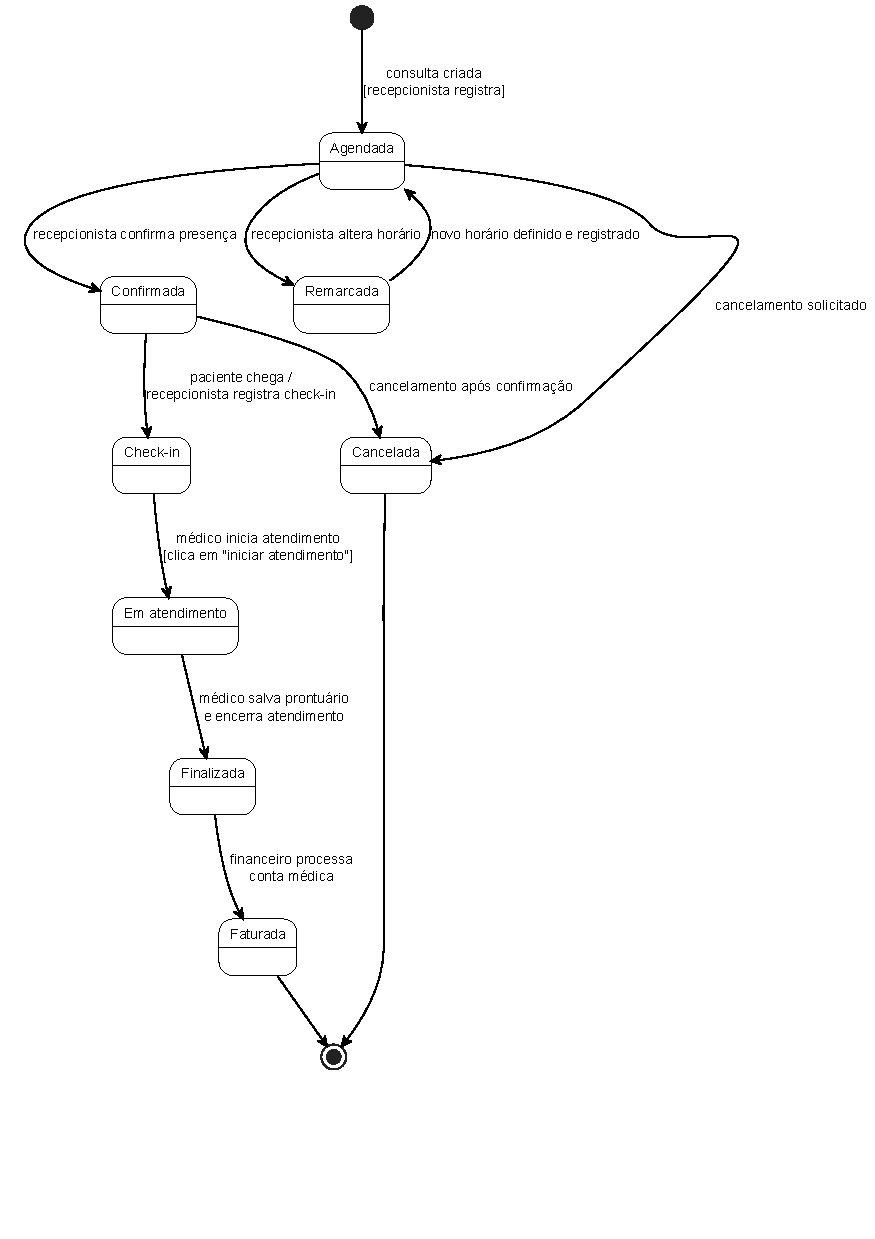
\includegraphics[
    width=0.85\linewidth,
    height=0.95\textheight,
    keepaspectratio
]{Imagens/arquitetura/DTE-ciclo-vida-consulta}

\caption{Ciclo de vida da entidade Consulta.}
\label{fig:dte-ciclo-vida-consulta}

\end{figure}

% ---------------------------------------------------------
% DTE — Prescrição
% ---------------------------------------------------------
\subsection{Ciclo de Vida de uma Prescrição}

O diagrama a seguir modela o ciclo de vida da entidade \texttt{Prescricao} no SGC. A partir do estado \textit{Emitida}, gerado quando o médico confirma a prescrição ao término ou durante o atendimento, o fluxo pode avançar para \textit{Dispensada Parcialmente}, caso a farmácia realize a entrega de apenas parte dos itens prescritos, ou diretamente para \textit{Dispensada}, quando todos os itens são entregues de uma vez. Cancelamentos são permitidos enquanto nenhum ou apenas parte dos itens tiver sido dispensado. O estado \textit{Dispensada} e o estado \textit{Cancelada} conduzem ao estado final do ciclo.

\begin{figure}[htbp]
\centering

\begin{center}
\small
\renewcommand{\arraystretch}{1.3}
\begin{tabular}{ll}
\textbf{View}        & V1 --- Visão de Cenários \\
\textbf{Model Kind}  & UML State Diagram \\
\textbf{Concerns}    & C4 (Integridade Transacional), C5 (Auditoria), C10 (Persistência e Consistência) \\
\textbf{Decisões}    & DA06 (Transações Atômicas), DA07 (Auditoria Centralizada) \\
\end{tabular}
\end{center}

\vspace{1em}

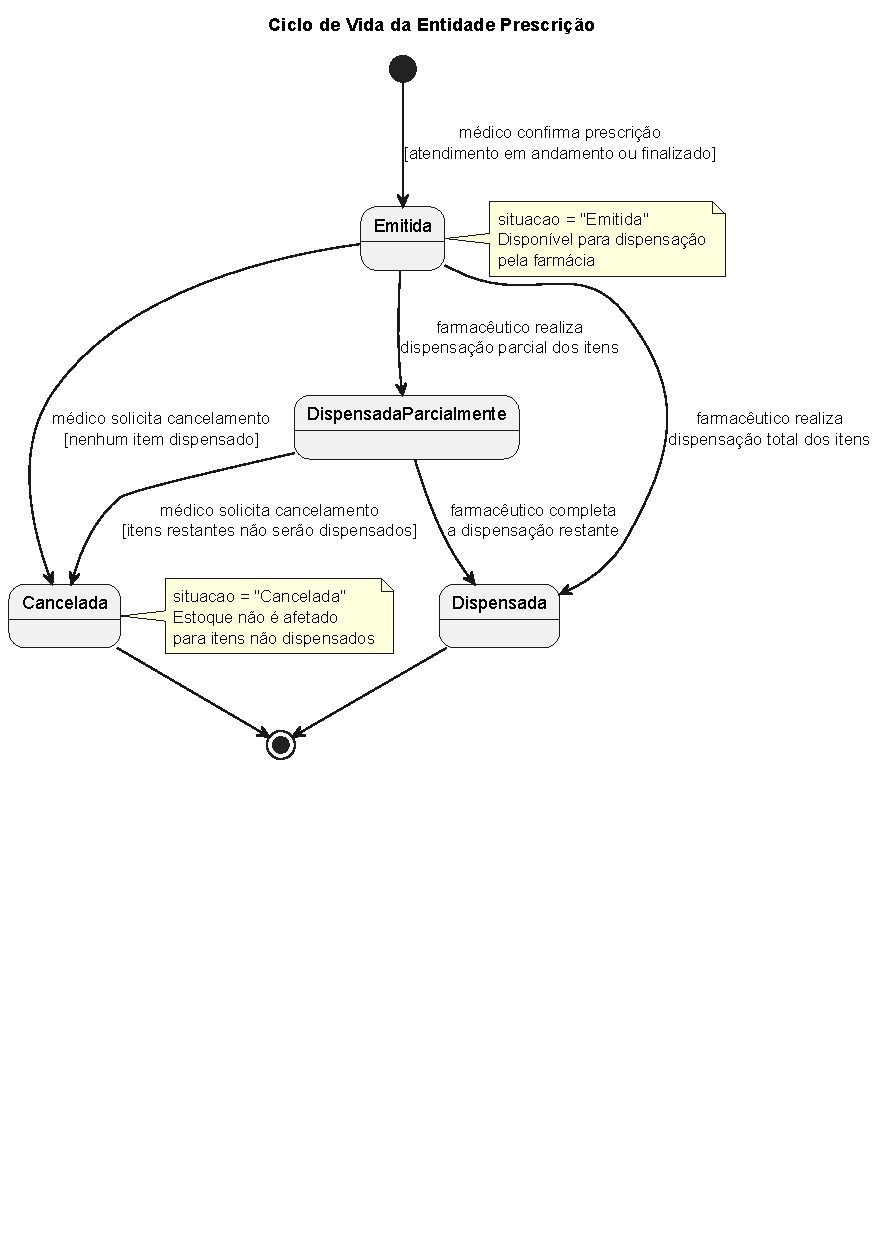
\includegraphics[
    width=0.75\linewidth,
    height=0.95\textheight,
    keepaspectratio
]{Imagens/arquitetura/DTE_Prescricao.pdf}

\caption{Ciclo de vida da entidade Prescrição.}
\label{fig:dte-ciclo-vida-prescricao}

\end{figure}


% ---------------------------------------------------------
% DTE — ContaMedica
% ---------------------------------------------------------
\subsection{Ciclo de Vida de uma Conta Médica}

O diagrama a seguir modela o ciclo de vida da entidade \texttt{ContaMedica} no SGC. A partir do estado \textit{Pendente}, gerado automaticamente após o processamento financeiro de uma consulta finalizada, a conta pode ser encaminhada para \textit{Em Análise} quando o convênio solicita revisão dos valores. Após a análise, os valores podem ser recalculados e a conta retorna a \textit{Pendente}, ou o convênio aprova e efetua o pagamento, conduzindo ao estado \textit{Pago}. Cancelamentos são permitidos a partir dos estados \textit{Pendente} e \textit{Em Análise}. Os estados \textit{Pago} e \textit{Cancelado} conduzem ao estado final do ciclo.

\begin{figure}[htbp]
\centering

\begin{center}
\small
\renewcommand{\arraystretch}{1.3}
\begin{tabular}{ll}
\textbf{View}        & V1 --- Visão de Cenários \\
\textbf{Model Kind}  & UML State Diagram \\
\textbf{Concerns}    & C4 (Integridade Transacional), C5 (Auditoria), C10 (Persistência e Consistência) \\
\textbf{Decisões}    & DA06 (Transações Atômicas), DA07 (Auditoria Centralizada) \\
\end{tabular}
\end{center}

\vspace{1em}

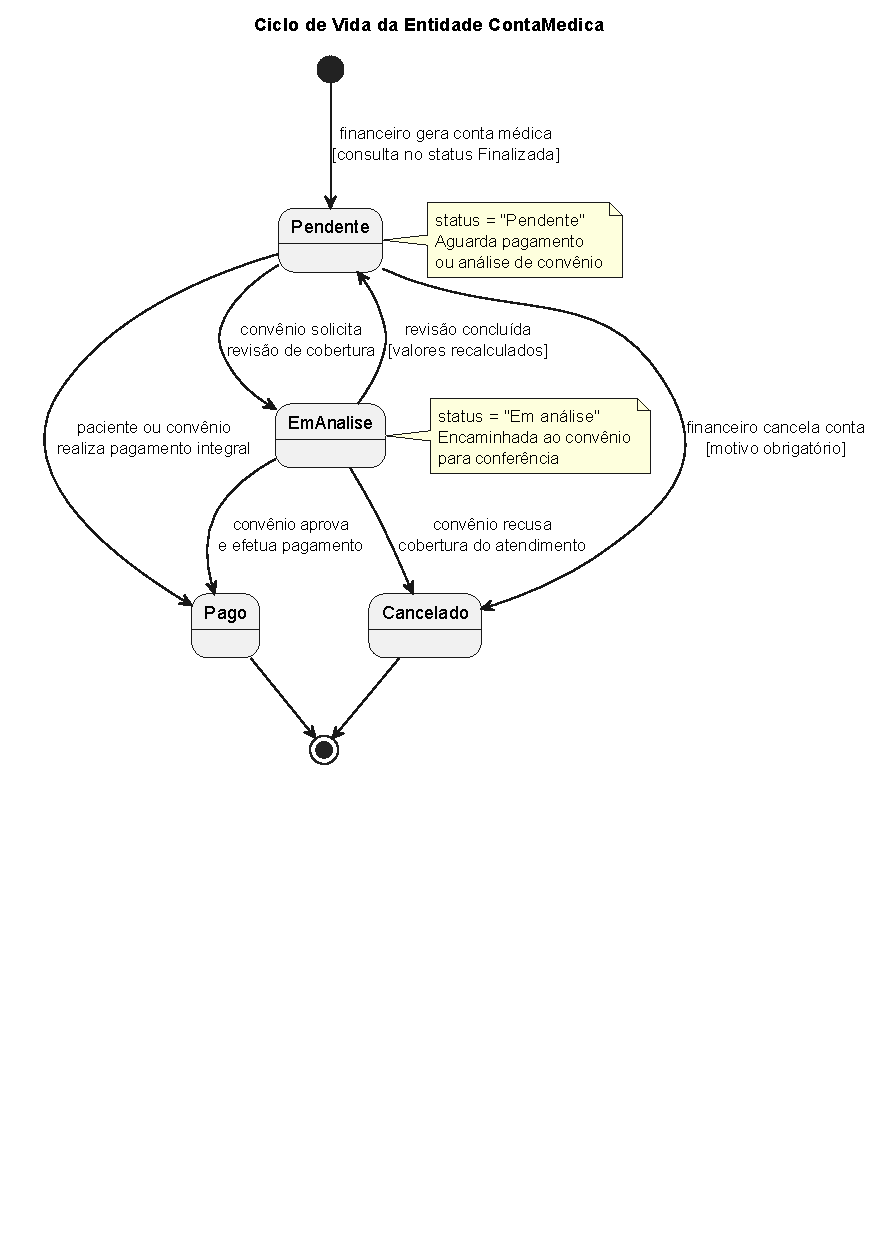
\includegraphics[
    width=0.75\linewidth,
    height=0.95\textheight,
    keepaspectratio
]{Imagens/arquitetura/DTE_ContaMedica.pdf}

\caption{Ciclo de vida da entidade ContaMedica.}
\label{fig:dte-ciclo-vida-conta-medica}

\end{figure}

% ---------------------------------------------------------
% Diagrama de Atividades
% ---------------------------------------------------------
\section{Diagrama de Atividades}

O diagrama de atividades é um fluxograma estendido que permite representar ações concorrentes, regras lógicas, sincronização e a divisão de tarefas por atores utilizando raias (\textit{swimlanes}).

\subsection{Processo de Triagem e Atendimento Clínico}

O diagrama a seguir descreve o processo colaborativo de triagem e atendimento clínico, baseando-se nos casos de uso UC02 (Gerenciar Agenda de Consultas), UC04 (Realizar Atendimento Clínico) e UC05 (Emitir Prescrição Médica). O fluxo é organizado em três raias (\textit{swimlanes}): \textbf{Recepcionista}, responsável pelo acolhimento do paciente e pelo registro do check-in; \textbf{Sistema (SGC)}, que valida a presença, atualiza o status da consulta e disponibiliza o prontuário na fila médica; e \textbf{Médico}, que conduz o atendimento clínico, preenche a evolução e decide sobre a necessidade de prescrição ou exames. Uma bifurcação lógica determina se a consulta gera ou não uma prescrição vinculada, após o que o médico confirma o encerramento e o sistema atualiza o status da consulta para \textit{Finalizada}.


\begin{landscape}
\thispagestyle{plain}

\begin{center}
\begin{minipage}{0.98\linewidth}

\begin{center}
\small
\renewcommand{\arraystretch}{1.2}
\begin{tabular}{lp{0.75\linewidth}}
\textbf{View}        & V1 --- Visão de Cenários \\
\textbf{Model Kind}  & UML Activity Diagram \\
\textbf{Concerns}    & C2 (Desempenho), C4 (Integridade Transacional), C9 (Usabilidade) \\
\textbf{Decisões}    & DA01 (Arquitetura em Camadas), DA06 (Transações Atômicas) \\
\end{tabular}
\end{center}

\vspace{0.6em}

\centering
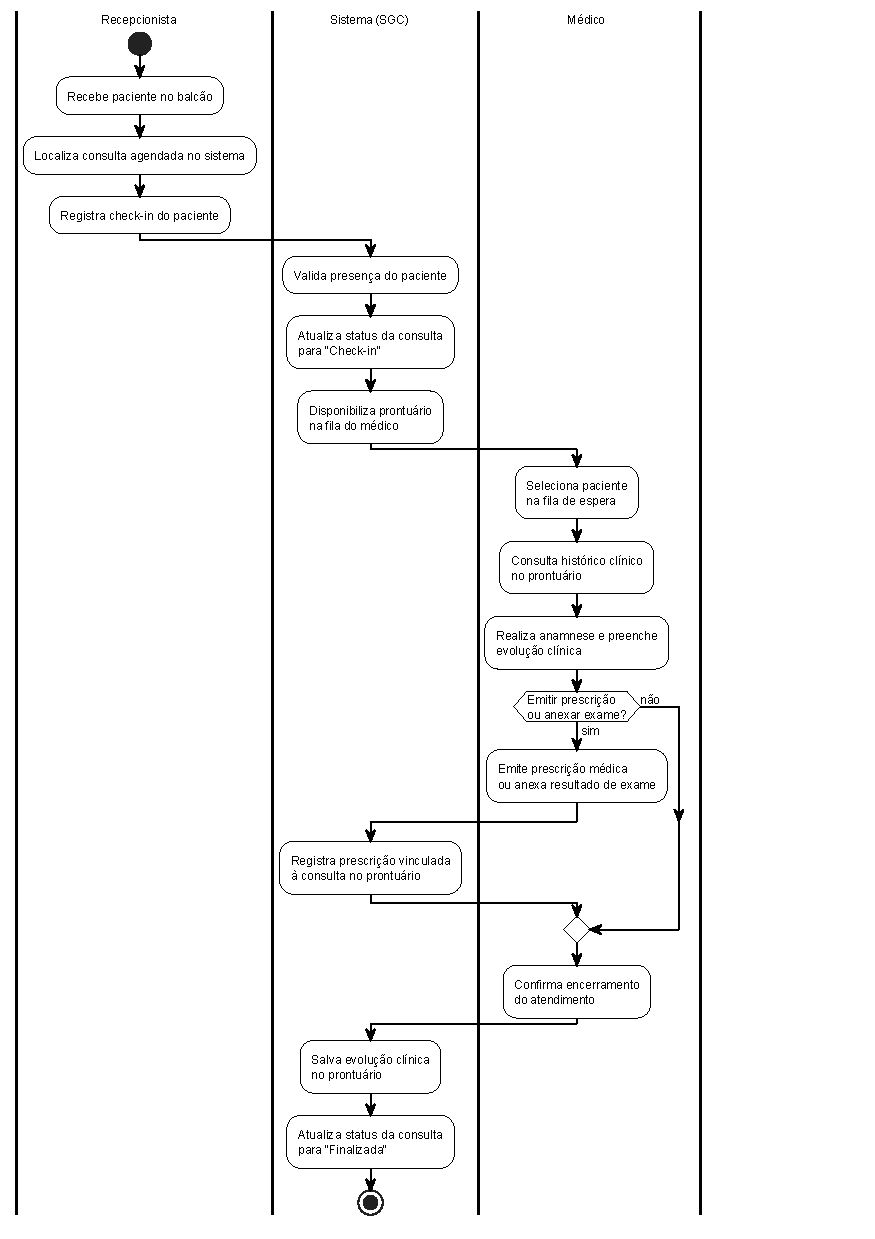
\includegraphics[
    width=0.98\linewidth,
    height=0.82\textheight,
    keepaspectratio
]{Imagens/arquitetura/DA-triagem-atendimento}

\captionof{figure}{Diagrama de atividades -- Processo de triagem e atendimento clínico.}
\label{fig:da-triagem-atendimento}

\end{minipage}
\end{center}

\end{landscape}
